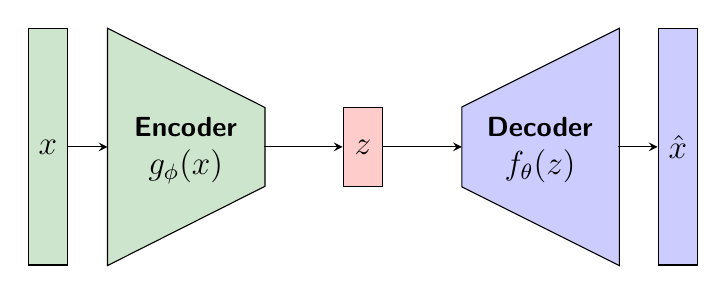
\begin{tikzpicture}
	%\node at (0.0,2.0){\begin{tabular}{c}{\sf Inputs} \end{tabular}};
	%\node at (8.0,2.0){\begin{tabular}{c}{\sf Reconstructed \\ \sf Inputs} \end{tabular}};
	
	\node[fill=Green!20, minimum width=0.5cm, minimum height=3.0cm, draw] (x) at (0,0) {\large $\boldsymbol x$};
	
	\draw[fill=Green!20] ([xshift=0.5cm]x.north east) -- ([xshift=2.5cm,yshift=0.5cm]x.east) -- ([xshift=2.5cm,yshift=-0.5cm]x.east) -- ([xshift=0.5cm]x.south east) -- cycle; 
	\node at (1.75,0.25) {{\sf \textbf{Encoder}}};
	\node at (1.75,-0.25) {\large $g_{\boldsymbol{\phi}}(\boldsymbol{x})$};
	
	\node[fill=red!20, minimum width=0.5cm, minimum height=1.0cm, draw] (z) at (4.0cm,0.0) {\large $\boldsymbol z$};
	
	\draw[fill=blue!20] ([xshift=1.0cm]z.north east) -- ([xshift=3.0cm,yshift=1.0cm]z.north east) -- ([xshift=3.0cm,yshift=-1.0cm]z.south east) -- ([xshift=1.0cm]z.south east) -- cycle;
	\node at (6.25,0.25) {{\sf \textbf{Decoder}}};
	\node at (6.25,-0.25) {\large $f_{\boldsymbol{\theta}}(\boldsymbol{z})$};
	
	\node[fill=blue!20, minimum width=0.5cm, minimum height=3.0cm, draw] (xhat) at (8.0cm,0) {\large $\boldsymbol{\hat{x}}$};
	
	\draw[-stealth] (x.east) -> ([xshift=0.5cm]x.east);
	\draw[-stealth] ([xshift=-1.0cm]z.west) -> (z.west);
	\draw[-stealth] (z.east) -> ([xshift=1.0cm]z.east);
	\draw[-stealth] ([xshift=-0.5cm]xhat.west) -> (xhat.west);
\end{tikzpicture}